\cleardoublepage%

\chapter{\label{chap:gen}Event Simulation}%
%\noindent Following the description of the particle composition of the SM and the theoretical construction of their interactions, this section introduces a phenomenological description of p-p collision physics and explains the concepts used to model collision events with characteristics comparable to real measurement conditions at the LHC. In the high-energy collisions further particles are created as a result of a hard interaction of the partons from both protons. In particular, the cross section of the particle production is a convolution of the structure of both protons and a partonic cross section. More thorough reviews of hadron collider physics is available in Refs.\\

\noindent In order to compare the data to predictions of the Standard Model (or of some other theory), samples are simulated using the Monte Carlo (MC) method to represent the stochastic effects and the probabilistic nature of the underlying theory. For this reason the simulated samples are often called Monte Carlo samples and the tools used to produce them are MC event generators.\\
\indent Their production is a complicated process, divided into two major steps. First, the underlying collision needs to be described, starting with the two protons in the initial state and their interaction and ending with stable particles in the final state. In the second stage, the propagation of particles from the first stage, through the detector and simulation of detector response needs to be performed. Each collision and its subsequent products constitute a single event and the production of the MC samples can be called an event simulation or generation.\\
\indent The simulation starts at small distances, where the colliding protons can be viewed as collections of partons (quarks and gluons). An interaction of these partons can lead to a hard-scattering, represented by a matrix element of the process. This is described in Section \ref{sec:ME_calculations}. In Section \ref{subsec:Higher_QCD} a brief overview of  next-to-leading-order calculations is presented while in Section \ref{sec:PS} the basics of parton showers are emphasized. These two complementary approaches for calculating higher orders can be combined into a common framework (NLO+PS). This is described in Section \ref{sec:NLO+PS}. In Section \ref{sec:MC_method} a short summary of the Monte Carlo methods used by the generators is presented. Finally, in Section \ref{sec:pp_collisions} the structure of a simulated event in a proton-proton collision is described.



% Notes: https://arxiv.org/pdf/hep-ph/0611247.pdf
% \indent The main motivation for constructing Monte-Carlo event generators is the need to make theoretical predictions for high-energy reactions in contemporary collider experiments, like those happening in LHC. Almost all of these reactions involve hadrons, either because the colliding particles are hadrons or because hadrons are produced in the final state and are thus used to define observables. However, these reactions cannot be directly predicted from first principles. Only their constituents, quarks and gluons, can be described as the quanta of QCD. Due to the asymptotic freedom, these partons can only then be regarded as free particles if they participate in a scattering process involvinf large inavriant momentum transfer and correspondinlgy short time scales. In such a case, like at the LHC, QCD allows to describe the interaction of partons using perturbation theory.\\
% \indent At higher orders in the perturbative expansion, such calculation predict infrared divergences of both, real-radiation and virtual contributions. Due to KLN-theorem, these divergences must mutually cancel for an inclusive cross section calculation. However,  if measurements or predictions have to be made more exclusively at a certain resolution scale, e.g. the hadronization scale, the divergences turn into a finite remainder which has a logarithmic dependence on the ratio between the hard scale and the resolution scale. Such potentially large logarithms will appear to each order in perturbation theory and thus spoil the convergence of the perturbative series, which is normally guaranteed by the smallness of the coupling constant. They must therefore be resummed to all orders. Such a resummation can be done analytically or by a numerical method called a parton-shower Monte Carlo.


% https://iopscience.iop.org/article/10.1088/1126-6708/2007/11/070/pdf





\section{Matrix element calculations in perturbative QCD} \label{sec:ME_calculations}
\noindent The principal task of QCD calculations for collider experiments is to relate the incoming state to the outgoing state. This is accomplished by the scattering matrix, which relates asymptotic incoming $\psi_{in}(\alpha)$ and outgoing states $\psi_{out}(\beta)$, described by the set of momenta and quantum numbers $\alpha$ and $\beta$, through the relation
\begin{equation}\label{eq:S_matrix}
    S_{\beta\alpha} \equiv \langle\psi_{out}(\beta)|\psi_{in}(\alpha)\rangle
\end{equation}
In QCD, $\psi_{in}$ and $\psi_{out}$ would in principle correspond to incoming and outgoing quarks and gluons, however complications arise due to the confining nature of the strong force. This complication is overcome via the factorization theorem that will be discussed in Section \ref{subsec:PDF}. For the moment we can pretend that the fields appearing in Equation (\ref{eq:S_matrix}) are the fundamental degrees of freedom of the theory, i.e. quarks and gluons.\\
\indent The $S$ matrix comprises of a trivial part (no interaction) and a non-trivial part
\begin{equation}\label{eq:S_matrix_2}
    S_{\beta\alpha} = \delta_{\beta\alpha} + iT_{\beta\alpha} = \delta_{\beta\alpha} + (2\pi)^4\delta^{(4)} \bigg(\sum_i p_i - \sum_f p_f\bigg)i \mathcal{M}_{\beta\alpha}
\end{equation}
The invariant matrix element $\mathcal{M}$ represents the non-trivial part of the scattering matrix, i.e. it encapsulates the dynamics of the interaction. The delta function in Equation (\ref{eq:S_matrix_2}) imposes the conservation of the incoming 4-momenta $p_i$.\\
\indent The matrix element can be calculated by perturbation theory using the QCD Feynman rules, which are derived from the QCD Lagrangian \cite{Perturbative_QCD}. Cross-sections can then be calculated using the so-called Fermi's golden rule \cite{48}, which states that the transition probabilities from one state to another are given by the squared amplitude of the matrix element describing the transition, multiplied by the density of final states. More specifically, for a process $p_1p_2 \rightarrow k_1 \dots k_n$, the cross section is given by
\begin{equation}\label{eq:dsigma}
    d\sigma = \frac{1}{F}|\mathcal{M}_n|^2d\Phi_n
\end{equation}
where $F$ is the incoming particle flux and $d\Phi_n$ is the n-particle final state phase space,
\begin{equation}
\begin{gathered}
    d\Phi_n(q;k_1,\dots k_n) = (2\pi)^4 \delta^{(4)}\bigg(q - \sum_{i=1}^n k_1\bigg) \prod_{i=1}^n \frac{d^3k_i}{(2\pi)^32k_i^0} \\
    F = 4\sqrt{(p_1 \cdot p_2)^2 - (m_1 m_2)^2}
    \end{gathered}
\end{equation}
\subsection{Factorization and parton distribution functions}\label{subsec:PDF}
\noindent It was first proposed by Feynman \cite{Feynman_51}, that lepton-hadron scattering in the limit of large momentum transfer can be explained by the parton model. In this model, the hadron is viewed as consisting of fundamental point-like constituents, which were later identified as QCD quarks and gluons. As it was further elaborated by Bjorken and Paschos \cite{Bjorken_52}, the essential ingredient of the parton model is to consider a class of infinite momentum frames, in which a parton $i$ will carry a fraction $0<x_i<1$ of the hadron's momentum. Consequently, the hadronic cross section $\sigma_{pp\rightarrow X}$ could be obtained by convolving the cross-section for the hard-scattering sub-process $\hat{\sigma}_{ij\rightarrow X}$ with the Parton Distribution Functions (PDFs) $f_i$,
\begin{equation}\label{eq:sigma_2}
    \sigma_{pp\rightarrow X} =\sum_{ij} \iint dx_i dx_j f_i(x_i, \mu_F^2)f_j(x_j,\mu_F^2)\hat{\sigma}_{ij\rightarrow X}(x_i,x_j, \mu_F^2, \mu_R^2)
\end{equation}

The PDFs $f_i(x, \mu_F^2)$ express the probability of finding a parton $i$ inside the hardon, in this case inside a proton, carrying a momentum fraction $x$. However, the perturbative calculation is limited at a certain threshold by the energy dependence of the strong coupling constant which is growing with decreasing energy. The non-perturbative parts factorize at a characteristic energy scale $\mu_F$ and are incorporated into the PDFs extracted from observed data. This energy scale is called the factorization scale and generally represents the smallest scale at which a physical process may be resolved and absorbed into the non-perturbative PDF. In addition, we have introduced another scale, $\mu_R^2$, called the renormalization scale which removes nonphysical divergences. Equation (\ref{eq:sigma_2}) is an example of theorems called factorization theorems \cite{55} which essentially express the fact that in certain kinematic regimes the non-perturbative dynamics, encapsulated in the PDFs, can be separated from the perturbative dynamics, encapsulated in the partonic cross section.\\
\indent However, these energy scales that we introduced are non-physical and in the case of an exact expansion of the perturbation series an observable $\mathscr{O}$ is independent of these parameters. This is expressed via the so-called renormalization group equation (RGE)
\begin{equation}
    \frac{\partial\mathscr{O}(x,Q^2)}{\partial\ln(\mu^2)}= \frac{\partial\mathscr{O}_{LO}}{\partial\ln(\mu^2)} + \frac{\partial\mathscr{O}_{NLO}}{\partial\ln(\mu^2)} + \sum_{k=2}^{\infty} \frac{\partial\mathscr{O}_{N^kLO}}{\partial\ln(\mu^2)} = 0
\end{equation}
In analogy with the beta function for the QCD running coupling, Equation (\ref{eq:beta_function}), the RGE leads to the evolution equations for the PDFs [49], which are known as the DGLAP\footnote{The acronym DGLAP refers to the names of its authors: Dokshitzer-Gribov-Lipatov-Altarelli-Parisi} equations \cite{56,57,58,59}
\begin{equation}
    \frac{d}{d\ln\mu_F^2} \begin{pmatrix}
        f_{q_i}(x, \mu_F^2) \\
        f_g(x,\mu_F^2)
    \end{pmatrix} = \sum_j \frac{\alpha_s}{2\pi}\int_x^1 \frac{d\xi}{\xi}\begin{pmatrix}
        P_{q_iq_j}\big(\frac{x}{\xi}\big) & P_{q_ig}\big(\frac{x}{\xi}\big) \\
        P_{gq_j}\big(\frac{x}{\xi}\big) & P_{gg}\big(\frac{x}{\xi}\big)
    \end{pmatrix}\begin{pmatrix}
        f_{q_j}(\xi,\mu_F^2) \\
        f_g(\xi, \mu_F^2)
    \end{pmatrix}
\end{equation}
The DGLAP equations express the fact that a quark or gluon with momentum fraction $x$ can come from a quark or gluon with a larger momentum fraction $x/\xi$ with a probability proportional to $\alpha_s  P_{ij}$. Here, $P_{ij}$ are the so-called splitting functions, which are calculable in perturbation theory, with the LO contributions shown in Figure \ref{fig:DGLAP}.

\begin{equation}\label{eq:splitiing_functions}
    \begin{gathered}
        P_{gg}(z) = 2 C_A\Bigg[\Bigg(\frac{z}{1-z}\Bigg)_+ + \frac{1-z}{z} + z(1-z)\Bigg] + \frac{11C_A - 4n_fT_f}{6}\delta(1-z) \\
        P_{qq}(z) = C_F \Bigg(\frac{1+z^2}{[1-z]}\Bigg)_+ \\
        P_{gq}(z) = C_F\bigg[\frac{1 + (1-z)^2}{z}\bigg] \\
        P_{qg}(z) = T_F\big[z^2 + (1-z)^2\big]         
    \end{gathered}
\end{equation}
where $C_F = 4/3$, $C_A = 3$ and $T_F = 1/2$, while the notation $_+$ indicates that we treat the splitting functions at $z=1$ as distribution functions. 
\begin{equation}
    F(z)_+ = F(z) - \delta(1-z)\int_0^1 d\zeta F(\zeta)
\end{equation}
Physically, this corresponds to the fact that as the momentum scale of the interaction is increased, the sea of quark-antiquark pairs and gluons that surround the original parton are resolved. We note that although the DGLAP equations determine the evolution of the PDFs with the energy transfer, the $x$-dependence, shown in Figure \ref{fig:PDF} for an example PDF set, can only be determined by data.\\
\begin{figure}[H]
    \centering
    \begin{subfigure}{0.32\textwidth}
        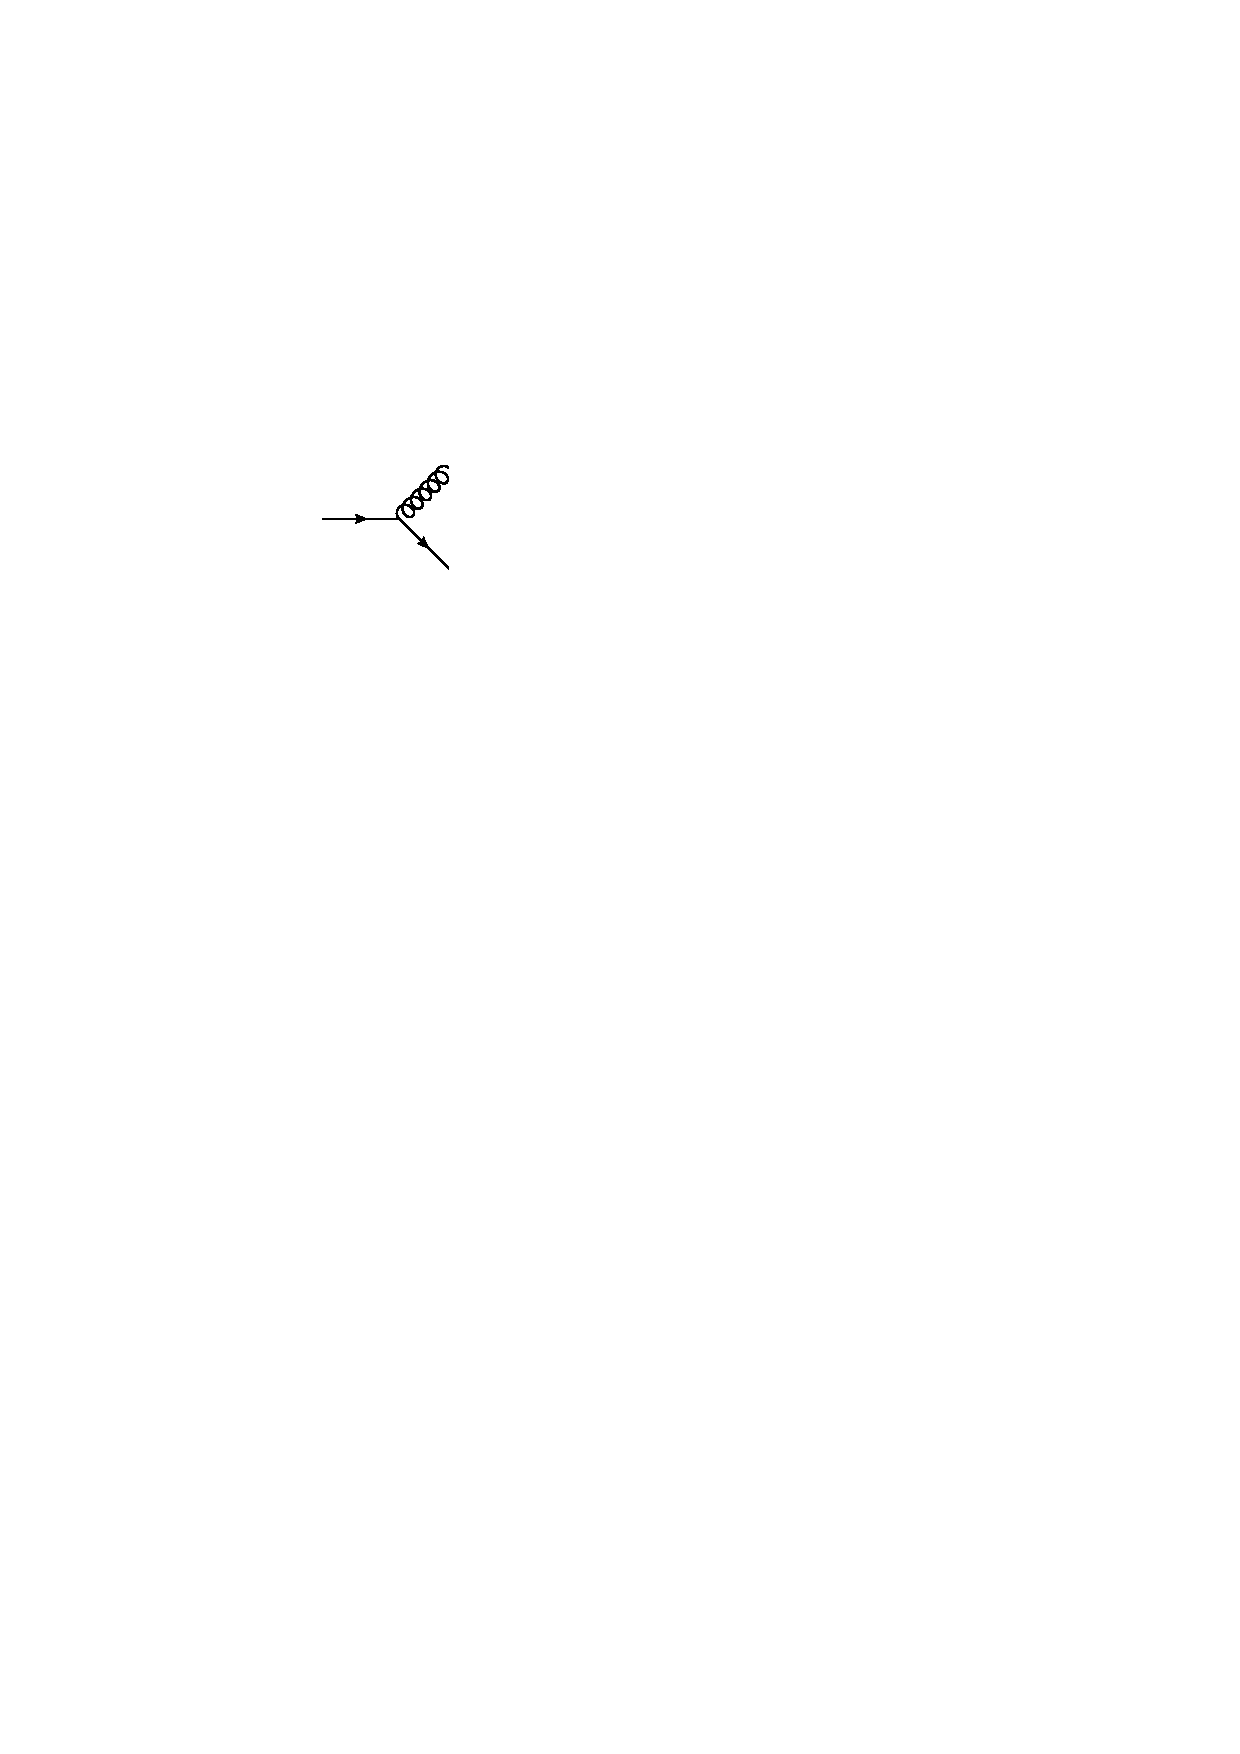
\includegraphics[width=0.8\linewidth]{Pqq.pdf}
        \caption{$P_{qq}$}
        \label{subfig:Pqq}
    \end{subfigure}
        \begin{subfigure}{0.32\textwidth}
        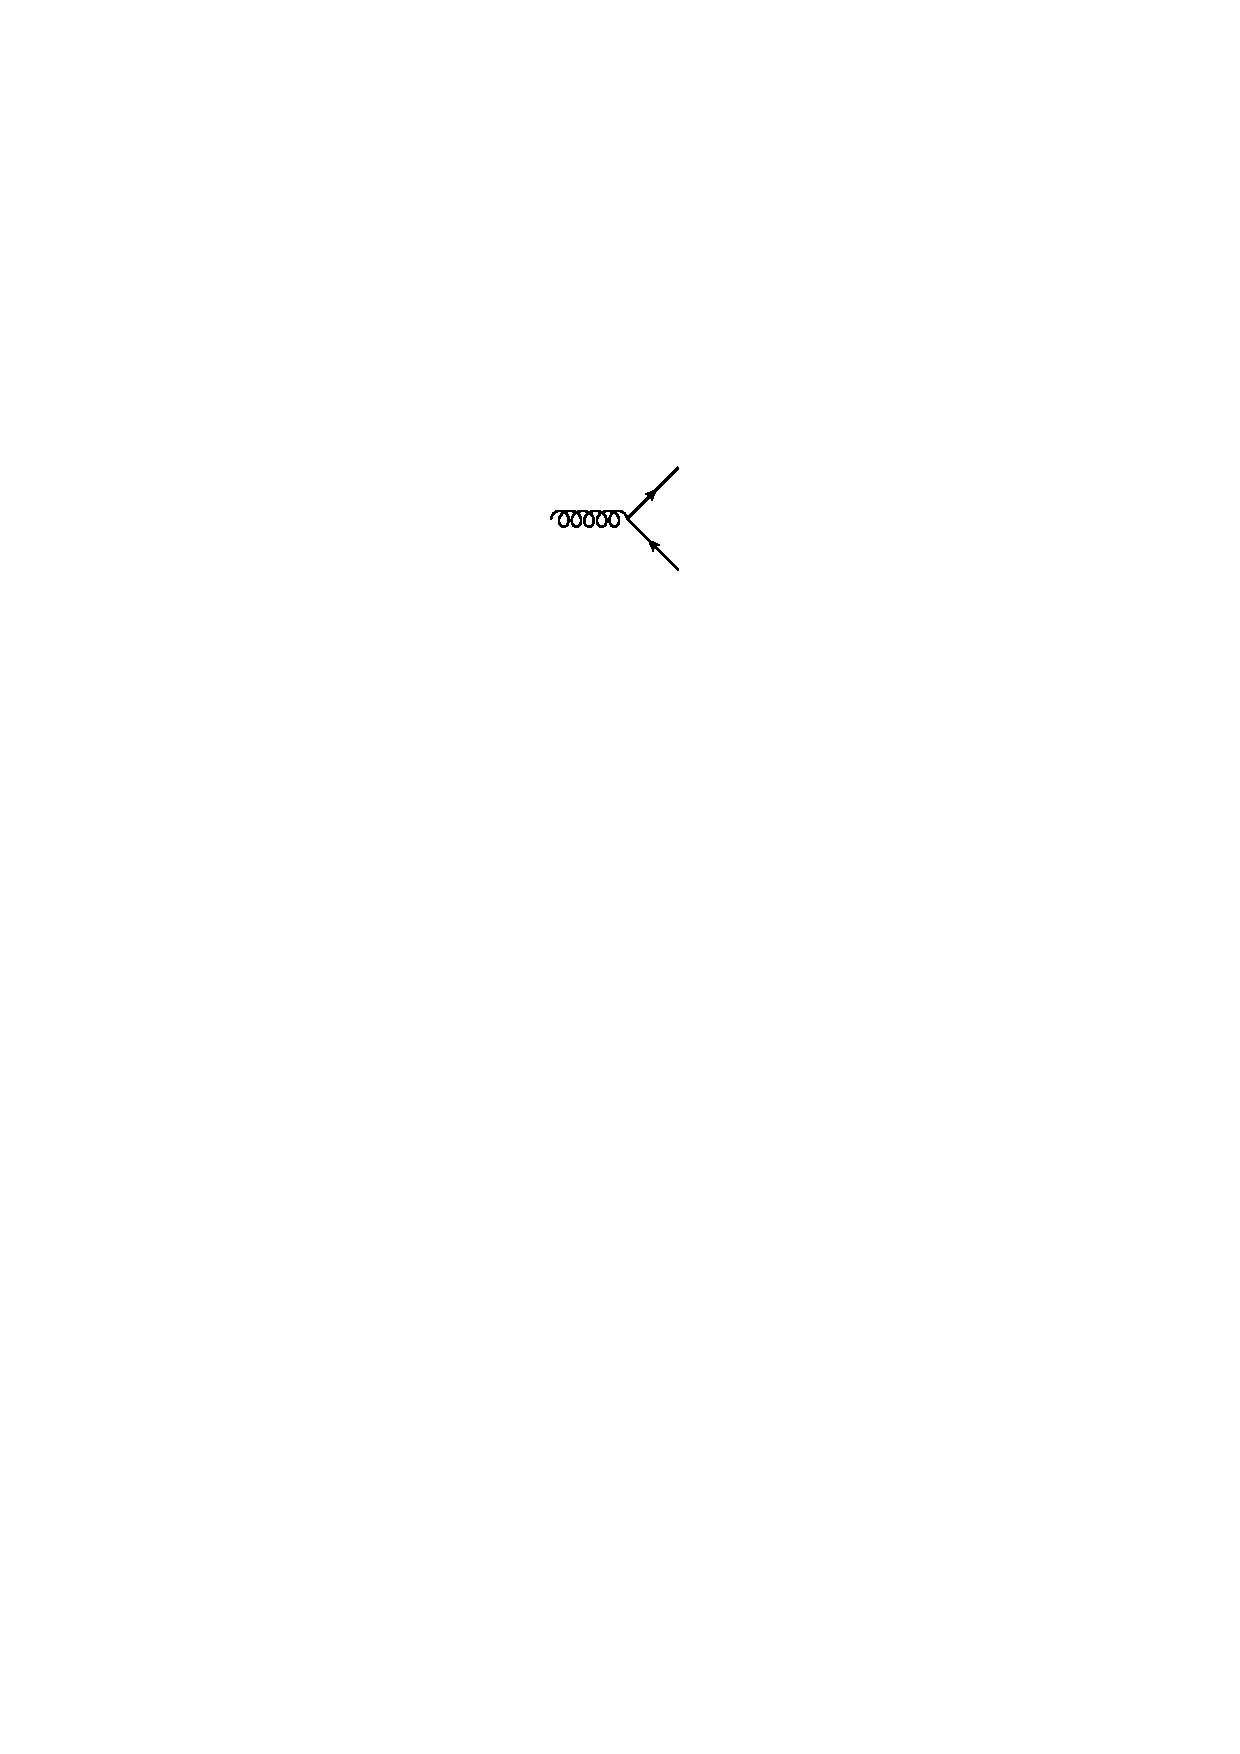
\includegraphics[width=0.8\linewidth]{Pqg.pdf}
        \caption{$P_{qg}$}
        \label{subfig:P_qg}
    \end{subfigure}
        \begin{subfigure}{0.32\textwidth}
        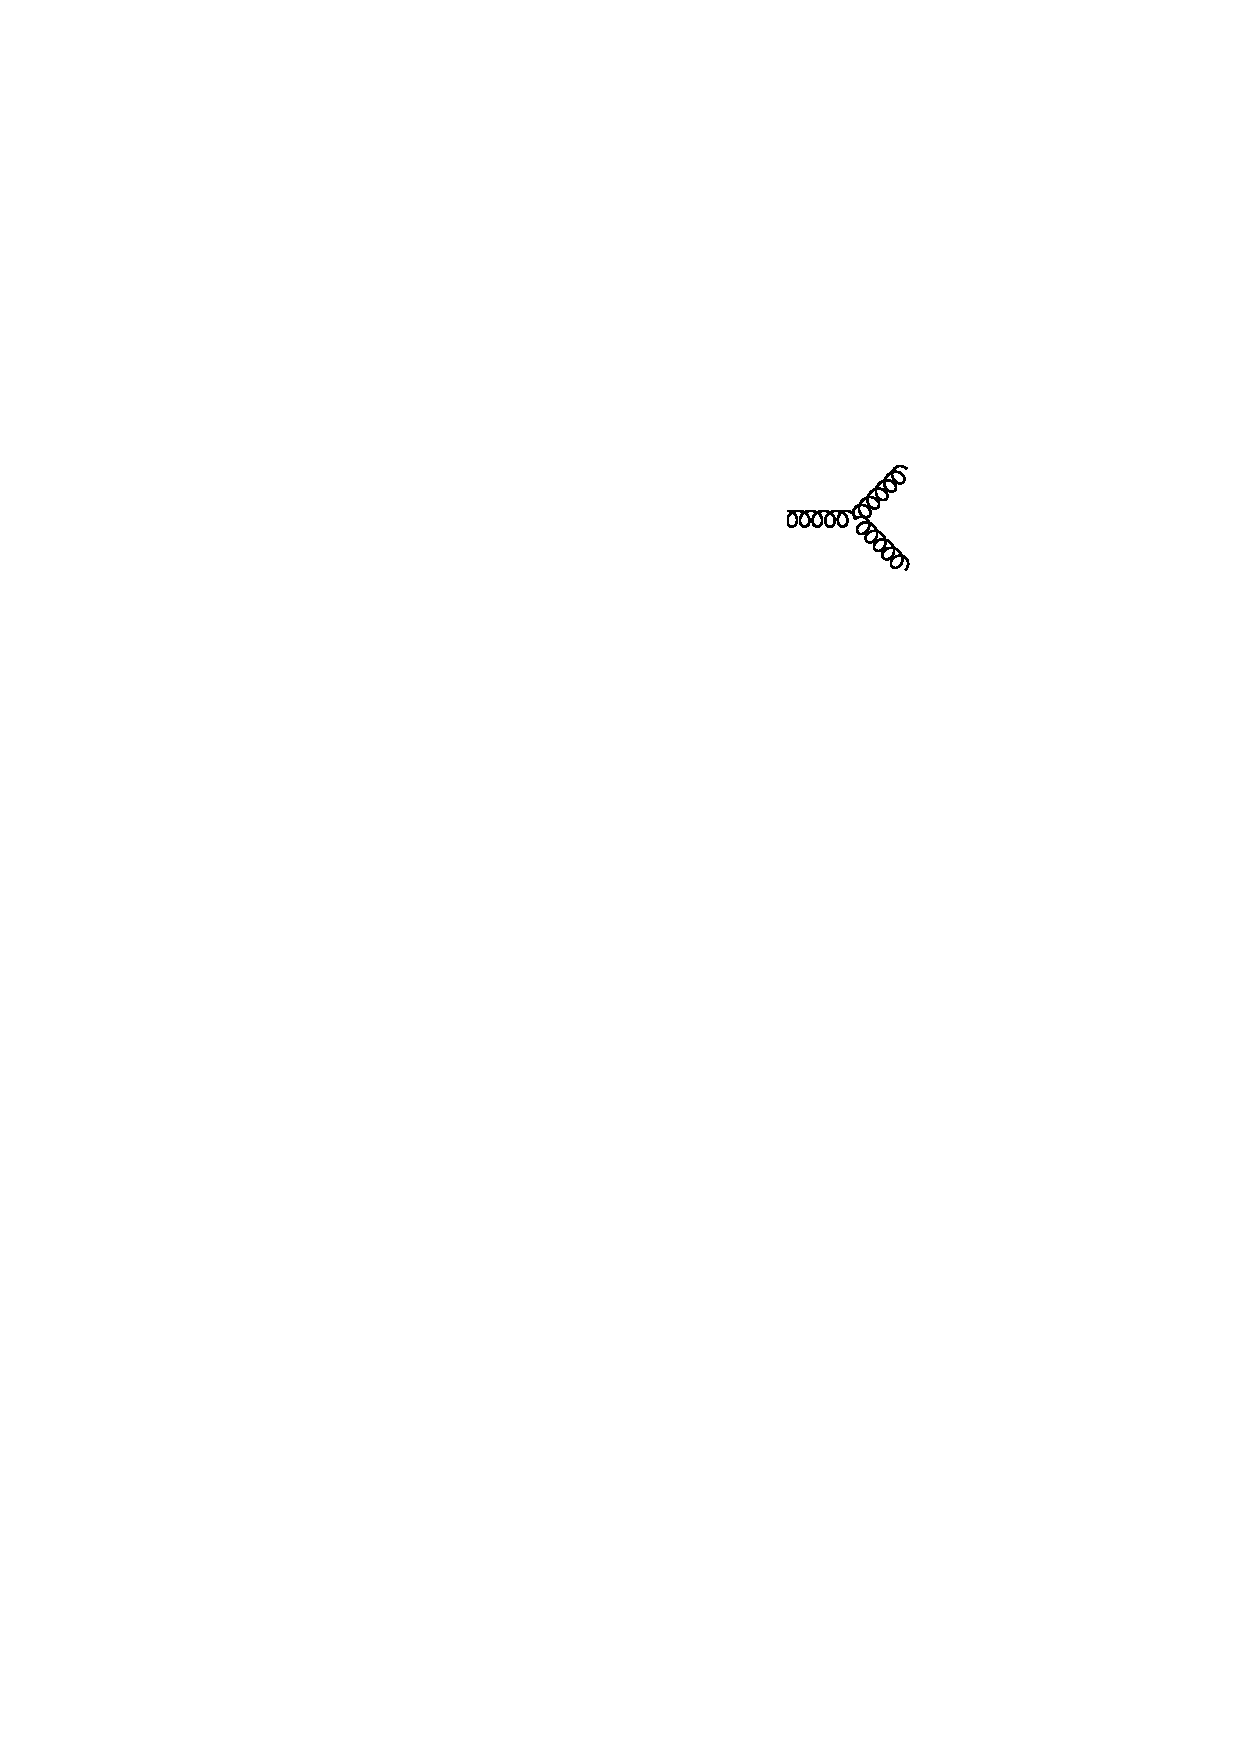
\includegraphics[width=0.8\linewidth]{Pgg.pdf}
        \caption{$P_{gg}$}
        \label{subfig:Pgg}
    \end{subfigure}
    \caption{LO contributions to the DGLAP splitting kernels}
    \label{fig:DGLAP}
\end{figure}
\indent Since an exact calculation is not possible, observables are usually calculated at leading-order (LO), next-to-leading-order (NLO) or next-to-next-to-leading-order (NNLO). The renormalization scale is normally chosen to be equal to the scale of the hard scattering process and is calculated individually for each event. The factorization scale is usually set to the same value as the renormalization scale. 
\begin{figure}[H]
    \centering
    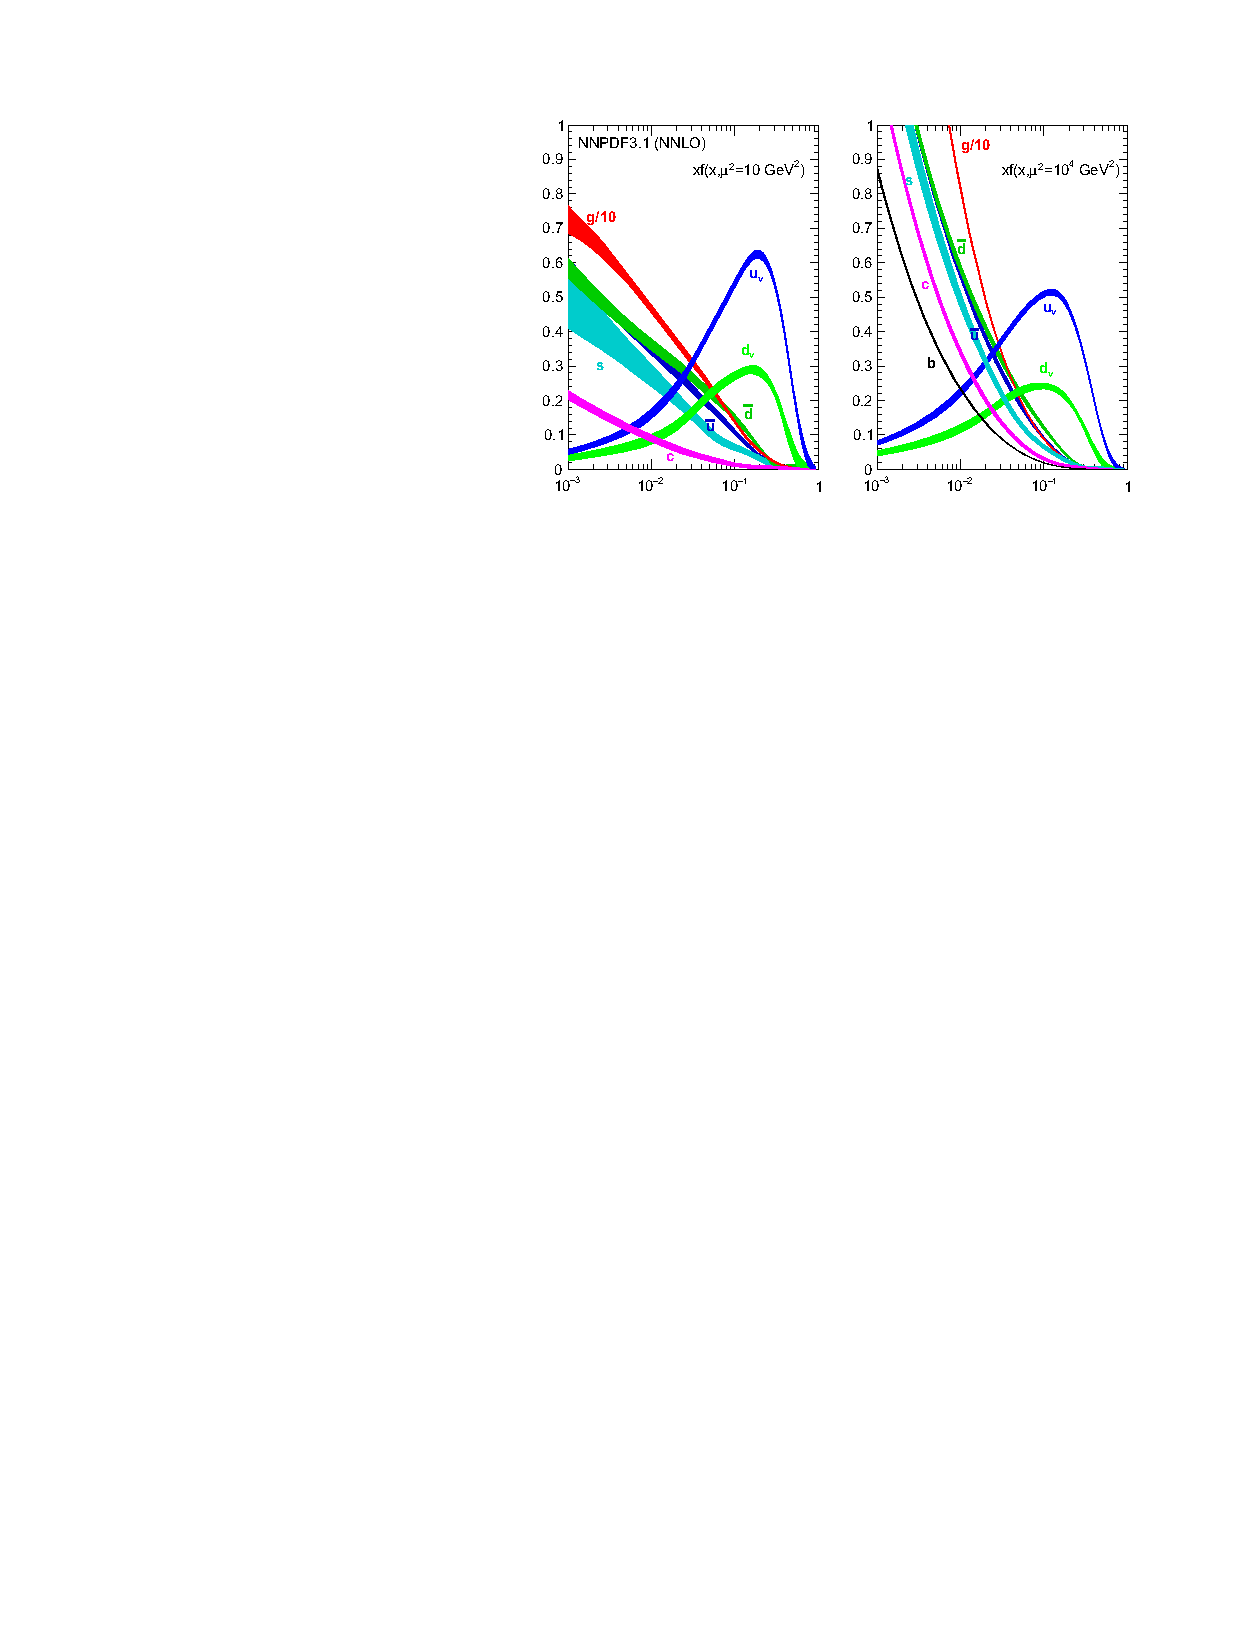
\includegraphics[width=0.9\linewidth]{Parton distributions from high-precision collider data_cropped_cropped.pdf}
    \caption{NNPDF3.1 NNLO pdf as a function of the momentum fraction $x$ of partons in a proton. The NNPDF3.1 NNLO pdf set is evaluated at two different scales $\mu_F^2$. On the left at lower energy scale $\mu_F^2 = 10 \text{GeV}^2$ and on the right at higher energy scale $\mu_F^2 = 10^4 \text{GeV}^2$. The gluon pdfs (red) are scaled by a factor of 1/10 as their contribution is by far dominant at low momentum fraction $x$ \cite{Ball2017}.}
    \label{fig:PDF}
\end{figure}

\subsection{Higher order QCD calculations}\label{subsec:Higher_QCD}
\noindent The matrix element in Equation (\ref{eq:dsigma}) has a perturbative expansion in $\alpha_s$. Going beyond the lowest order contributing to a given process corresponds to the emission or emission and re-absorption of gluons, as shown in Figure \ref{fig:NLO_contributions}. In the usual nomenclature, the tree-level contributions, i.e. containing no loops, are referred to as Born contributions, while $N^kLO$ contributions correspond
to adding k gluons to the LO contribution.
\begin{figure}[H]
    \centering
    \begin{subfigure}{0.32\textwidth}
        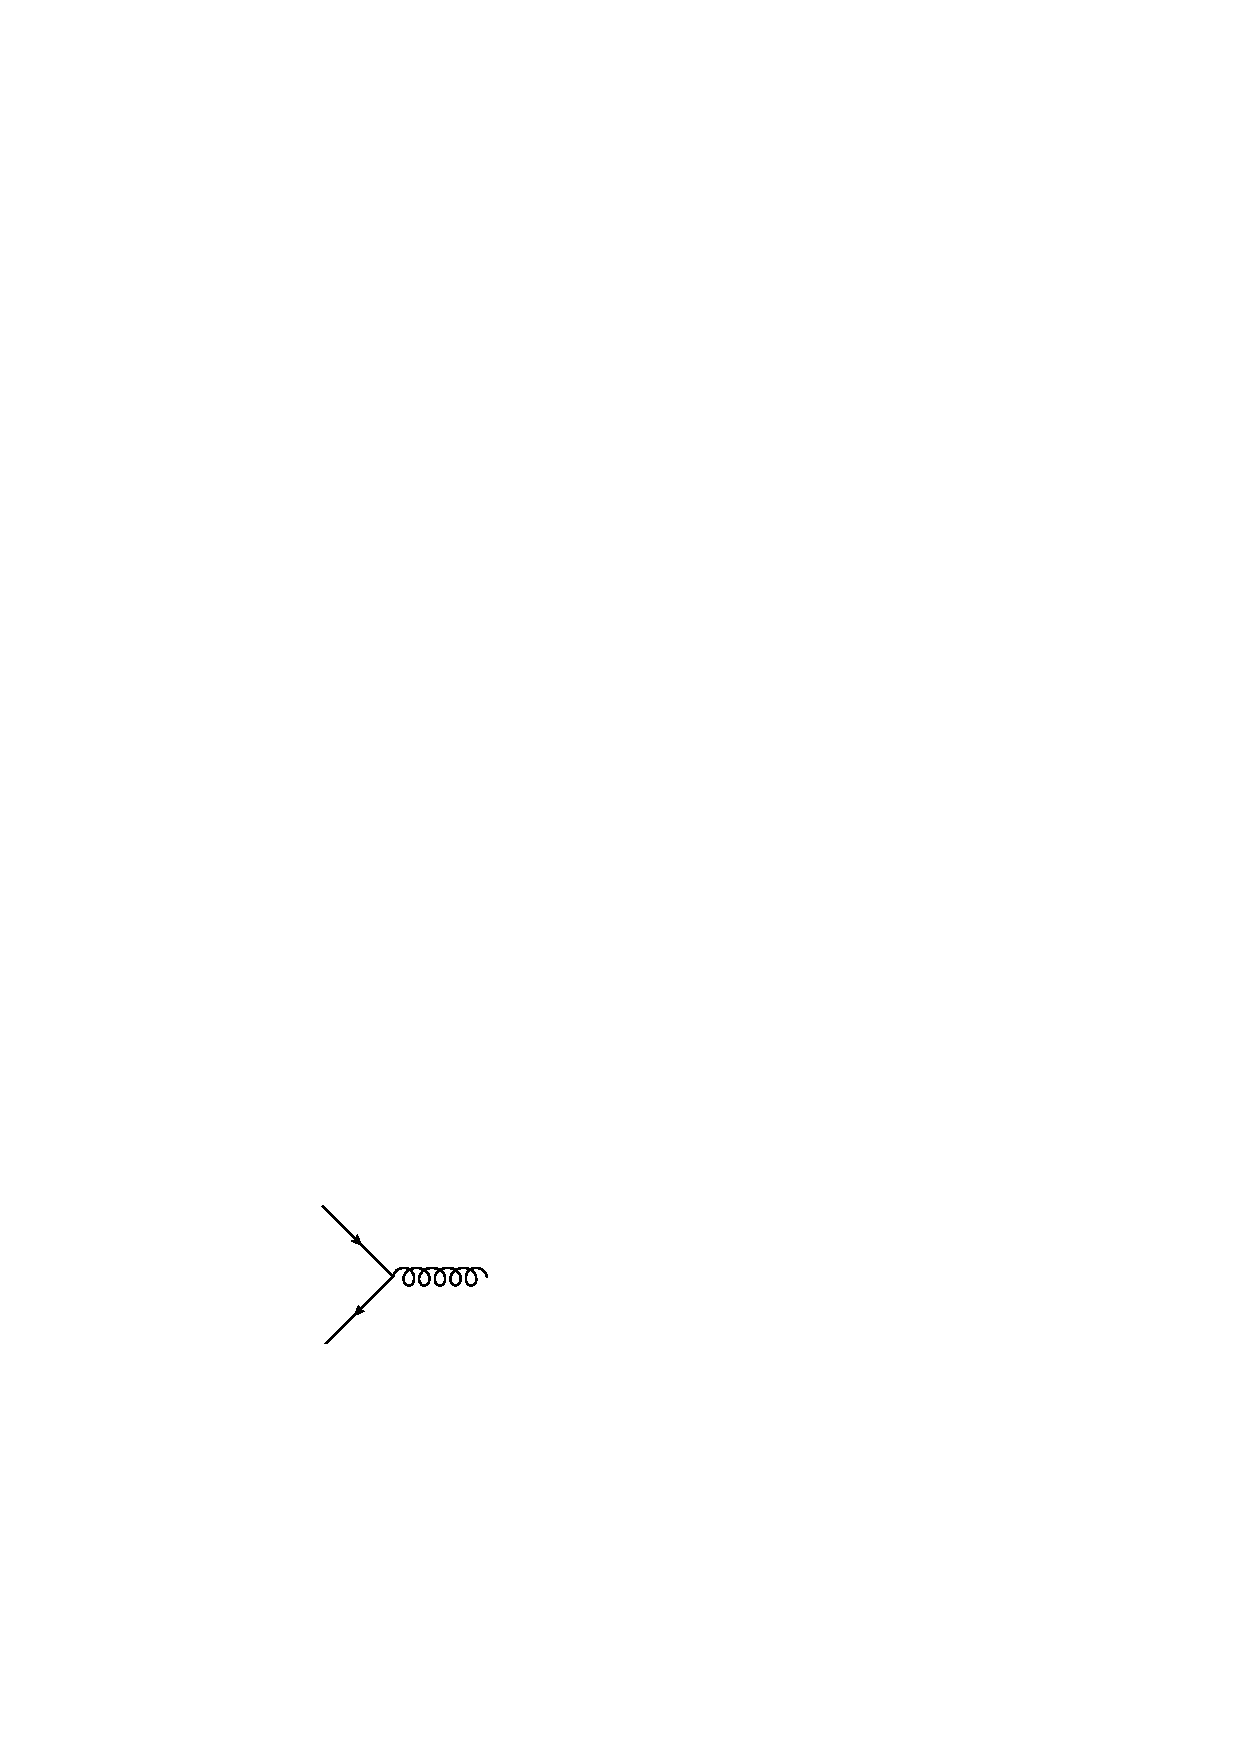
\includegraphics[width=0.9\linewidth]{Measurement of the ttbb production cross-section with 8 TeV ATLAS data_cropped2_cropped.pdf}
        
        \caption{}
        \label{subfig:Born}
    \end{subfigure}
        \begin{subfigure}{0.32\textwidth}
        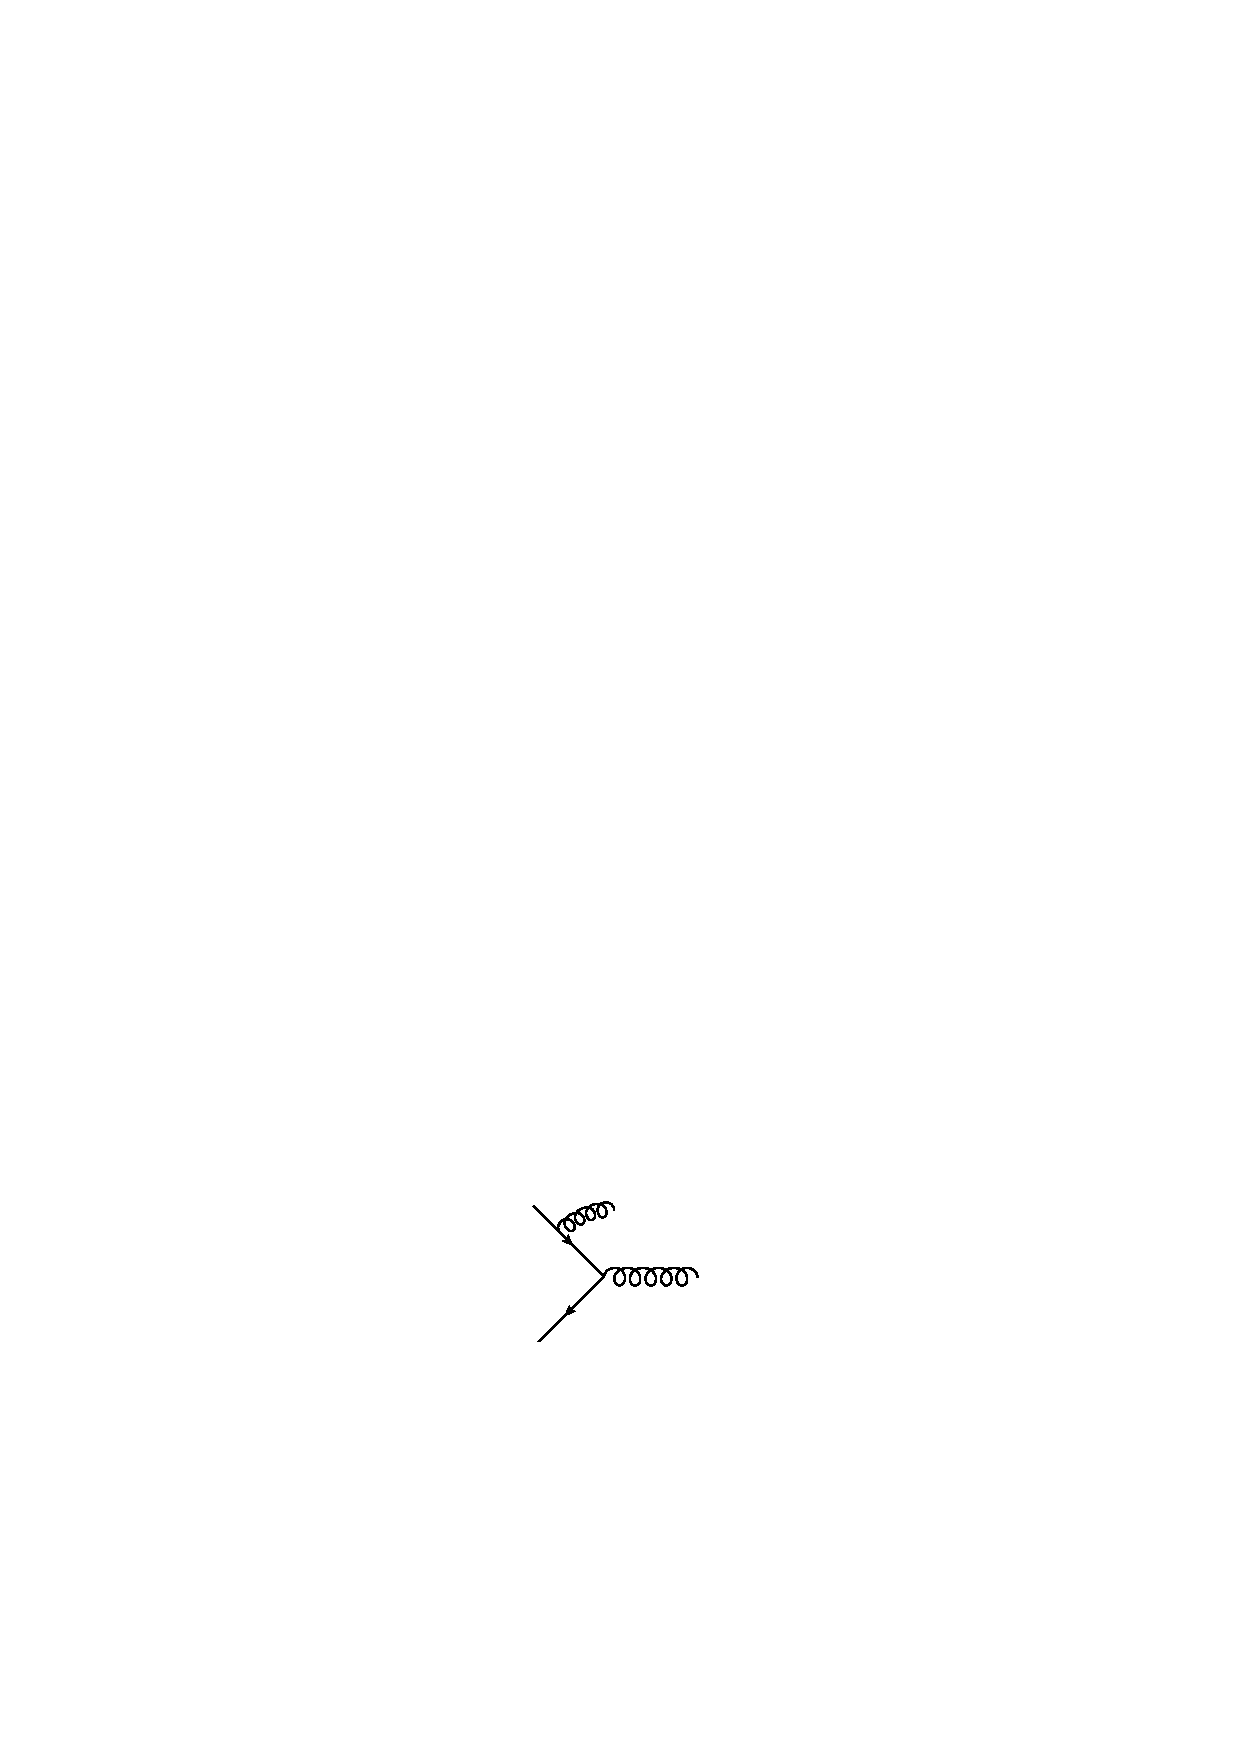
\includegraphics[width=0.9\linewidth]{Measurement of the ttbb production cross-section with 8 TeV ATLAS data_cropped2_2.pdf}
        
        \caption{}
        \label{subfig:Real}
    \end{subfigure}
        \begin{subfigure}{0.32\textwidth}
        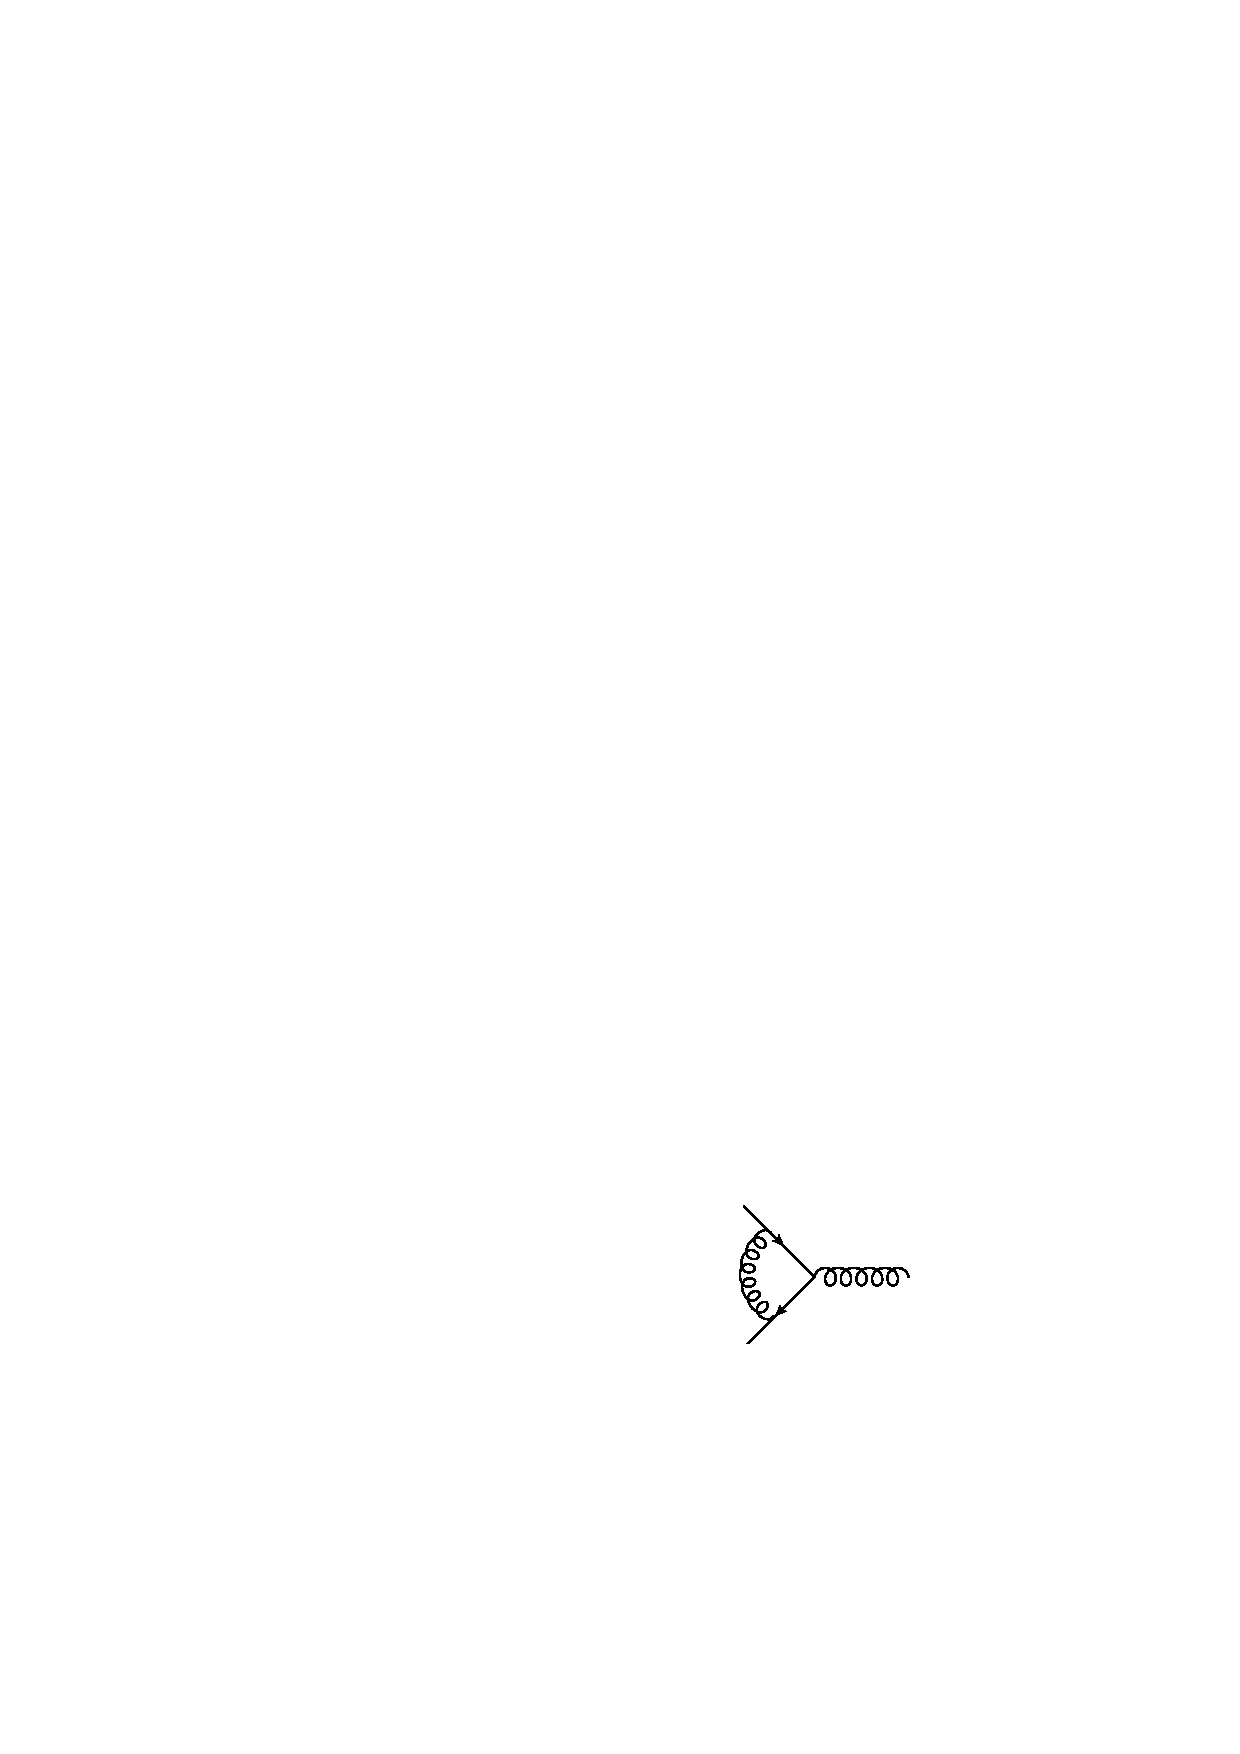
\includegraphics[width=0.9\linewidth]{Measurement of the ttbb production cross-section with 8 TeV ATLAS data_cropped2_3.pdf}
        
        \caption{}
        \label{subfig:Virtual}
    \end{subfigure}
    \caption{Example of (a) Born, (b) Real and (c) Virtual Feynman diagrams}
    \label{fig:NLO_contributions}
\end{figure}
One can symbolically write the parton-level cross-section at NLO accuracy as
\begin{equation} \label{eq:sigma_NLO}
    \sigma^{NLO} = \int_n d\sigma^B + \int_{n+1} d\sigma^R + \int_n d\sigma^V
\end{equation}
with $d\sigma^B, d\sigma^R, d\sigma^V$ representing the Born (LO), Real and Virtual contributions respectively while the integration subscripts represent the number of partons in the final state. The exclusive cross sections $d\sigma^R$ and $d\sigma^V$ have the same structure as the Born-level cross section in Equation (\ref{eq:dsigma}), apart from the replacements $|\mathcal{M}_n|^2 \rightarrow |\mathcal{M}_{n+1}|^2$, $d\Phi_n \rightarrow d\Phi_{n+1}$ and $|\mathcal{M}_n|^2 \rightarrow |\mathcal{M}_n|^2_{(1-loop)}$. Here $|\mathcal{M}_n|^2_{(1-loop)}$ denotes the QCD amplitude to produce $n$ final state partons evaluated in the one-loop approximation.\\
\indent Expressing the Born cross section as $Bd\Phi_B$ and the real cross section as $Rd\Phi_R$ we can write the differential NLO cross section schematically as
\begin{equation}
    d\sigma^{NLO} = \big[ B(\Phi_B) + \hat{V}(\Phi_B)\big]d\Phi_B + R(\Phi_R)d\Phi_R
\end{equation}
where we have also assumed that all phase space Jacobians needed to reproduce the Lorentz invariant phase space are absorbed into the definition of $B$, $\hat{V}$ and $R$. In addition, we write $d\Phi_R = d\Phi_Bd\Phi_{rad}$ where $\Phi_{rad}$ is the radiation phase space.\\
\indent However, the calculation of these integrals, leads to the so-called ultraviolet, infrared (soft) and collinear divergences. Ultraviolet divergences arise from the $p \rightarrow \infty$ limit of the loop integral, i.e. the virtual cross section. Infrared divergences come from the the $p \rightarrow 0$ limit of loop diagrams and the emission of soft gluons in the real contributions while the collinear divergences are from real emission diagrams which involve branchings between three massless partons. These divergences are not physical but signal the breakdown of perturbation theory. The ultraviolet divergences can be handled in a simple way within the loop corrections by carrying out the renormalization procedure, introducing $\mu_R$. Thus, we can assume that the virtual cross section in Equation (\ref{eq:sigma_NLO}) is given it terms of the renormalized matrix element and the ultraviolet divergences have been removed. On the other hand, infrared and collinear divergences lead to the main problem. Due to the Kinoshita-Lee-Nauenberg theorem \cite{61,62}, by adding the real and virtual contributions, must mutually cancel for an inclusive cross section calculation. However, this cancellation does not take place at the integrand level. \\
\indent The cancellation of soft and collinear divergences in NLO calculations is usually dealt with using the subtraction method \cite{Catani_1997}. The general idea of the subtraction method is to introduce an auxiliary counter-term $C(\Phi_R)$ which is required to coincide with the real squared amplitude $R$ in the soft and collinear limit:
\begin{equation}
    d\sigma^{NLO} = \big[ B(\Phi_B) + \hat{V}(\Phi_B)\big]d\Phi_B + \big[R(\Phi_R) - C(\Phi_R)\big]d\Phi_R + C(\Phi_R)d\Phi_R
\end{equation}
Assuming that we want to compute an infrared safe observable $\mathscr{O}$, the infrared safety requires that, in the soft or the collinear limit:  
\begin{equation}
    \mathscr{O}(\Phi_R(\Phi_B,\Phi_{rad})) \rightarrow \mathscr{O}(\Phi_B)
\end{equation}
Thus, we can write
\begin{equation} \label{eq:observable_subtraction}
    \begin{aligned}
        \langle\mathscr{O}\rangle &= \int d\sigma \mathscr{O} = \int d\Phi_B[B(\Phi_B) + \hat{V}(\Phi_B)]\mathscr{O}(\Phi_B) + \int d\Phi_R R(\Phi_R) \mathscr{O}(\Phi_R) \\
        &= \int d\Phi_B[B(\Phi_B) + V(\Phi_B)]\mathscr{O}(\Phi_B) + \int d\Phi_R [R(\Phi_R)\mathscr{O}(\Phi_R) - C(\Phi_R)\mathscr{O}(\Phi_B)]
    \end{aligned}
\end{equation}
where 
\begin{equation}\label{eq:virtual}
    V(\Phi_B) = \hat{V}(\Phi_B) + \int d\Phi_{rad} C(\Phi_R(\Phi_B, \Phi_{rad}))
\end{equation}
The above equations represent schematically the subtraction method in QCD. By suitable choice of the counter-term $C$, the integral of the radiation variables in Equation (\ref{eq:virtual})
can be performed analytically. The soft and collinear divergent terms arising from this integration cancel against those of the virtual term $\hat{V}$ yielding a finite result $V$. At the same time in Equation (\ref{eq:observable_subtraction}) the soft and collinear divergences in $R$ cancel, because in the soft or collinear limit $\mathscr{O}(\Phi_R) = \mathscr{O}(\Phi_B)$ and $C$ has the same singularity structure as $R$ \cite{Nason:2012pr}.

\section{The Parton Shower approach}\label{sec:PS}
\noindent Additional radiation can be described by the perturbative QCD framework up to the hadronization scale $\Lambda_{QCD}$, where the value of $\alpha_s$ becomes larger than one. However, due to an increasing number of contributing processes, current generators usually provide only a matrix element at the leading order or the NLO. Parton showers (PS) offer a way to generate the additional soft and collinear emissions, which dominate the production of additional particles. They are divided into the Initial State Radiation (ISR), connected to the initial parton from the proton before the hard scattering, and Final State Radiation (FSR), which describes emission from the particles produced by the hard scattering.\\
\indent We consider first the leading collinear region in which an extra parton is emitted at a small angle by one of the outgoing lines of an n-parton process (FSR). Here the cross section approximately factorizes in the form
\begin{equation}\label{eq:PS_1}
    d\sigma_{n+1}(\Phi_{n+1}) = \mathscr{P}(\Phi_{rad}) d\sigma_n(\Phi_n)d\Phi_{rad}
\end{equation}
and $d\Phi_{n+1} = d\Phi_nd\Phi_{rad}$. The function $\mathscr{P}$ depends on the type of emitting and emitted partons. In the notation of the previous Section, if the n-parton process is the Born process, we have $\Phi_n = \Phi_B$, $\Phi_{n+1} = \Phi_R$ and $\mathscr{P}(\Phi_{rad})B(\Phi_B) \equiv R^{(MC)}(\Phi_R)$ is an approximation to $R(\Phi_R)$ in the near-collinear region. In this region it is convenient to parameterize the phase space $\Phi_{rad}$ in terms of a hardness scale q, for example the transverse momentum $p_T$ or the angle $\theta$ relative to the emitter, the fraction of longitudinal momentum $z$ of the emitter after the emission and the azimuthial angle of splitting, $\phi$. Then,
\begin{equation}\label{eq:PS_2}
    \mathscr{P}(\Phi_{rad})d\Phi_{rad} \approx \frac{\alpha_s(q)}{\pi}\frac{dq}{q}P(z,\phi)dz\frac{d\phi}{2\pi}
\end{equation}
where $P(z,\phi)$ is the relevant splitting function, Equation (\ref{eq:splitiing_functions}), which in practise is averaged over the azimuthial angle and simply written as $P(z)$. The collinear divergence is regulated with a cutoff, $q > Q_0$. Emissions with $q < Q_0$ are said to be unresovable. Emissions with small momentum fractions $z$ are also unresolvable. Depending on the definition of the scale $q$, the cutoff on $z$ is some function $z_0(q,Q_0)$.\\
\indent Equations (\ref{eq:PS_1}) and (\ref{eq:PS_2}) provide the basis of an iterative scheme for summing collinear-enhanced contributions to all orders. Each parton participating in a hard process can emit at scales $q$ up to order $Q$. The probability of an emission in an interval between $q+dq$ and $q$ is given by Equation (\ref{eq:PS_2}). It follows that the probability of no resolvable emission between scales $q_1$ and $q_2 < q_1$ is given by
\begin{equation}
    \Delta_s(q_1,q_2) = exp\bigg[-\int_{q_2}^{q_1} \frac{a_s(q)}{\pi}\frac{dq}{q}\int_{z_0}^1P(z)dz\bigg]
\end{equation}
This function is known as the Sudakov form factor \cite{Sudakov:1954sw,Collins:1989bt}.\\
\indent The parton shower is generated in the following way:  for each particle $i$ at a scale $q$, a uniform random number $r$ between 0 and 1 is generated. One then finds a new scale $q_1$ by solving an equation $r = \Delta_s(q, q_1)$. If $q_1$ > $Q_0$ , a new emission is introduced at the scale $q_1$ otherwise the particle is considered to be a final state parton. This procedure is repeated until all partons are final state, producing new particles with a lower virtuality down to $Q_0$.\\
\indent A similar method is used also for the ISR \cite{Sjostrand:1985xi}. The only difference is that the initial partons have to be connected to the proton PDF leading to the formula:
\begin{equation}
    \mathscr{P}^{(ISR)}(\Phi_{rad})d\Phi_{rad} \approx \frac{\alpha_s(q)}{\pi}\frac{dq}{q}P(z)\frac{f(x/z,q)}{f(x,q)}dz\frac{d\phi}{2\pi}
\end{equation}
This obviously, leads to a different form of the Sudakov form-factor:
\begin{equation}
    \Delta_s^{(ISR)}(q_1,q_2) = exp\bigg[-\int_{q_2}^{q_1} \frac{a_s(q)}{\pi}\frac{dq}{q}\int_{z_0}^1P(z)dz\frac{f(x/z,q)}{f(x,q)}\bigg]
\end{equation}
\section{Matching NLO calculations with PS}\label{sec:NLO+PS}
\noindent Based on our earlier discussion, it's evident that there are two different approaches for the calculation of observables in hadron collisions: the matrix element approach which relies on perturbative calculations performed at a given fixed order and the parton shower approach which includes all-order contributions in the collinear limit. The two approaches are complementary in the sense that in the soft/collinear region, where the parton shower approach is valid, the matrix-element calculation breaks down due to the appearance of large logarithms, while in the hard/wide-angle emission region, where the matrix-element calculation provides a good description, the approximations involved in the parton shower approach become invalid.
\indent There are two methods for matching NLO matrix elements with parton showers, dubbed MC@NLO \cite{Frixione_2002} and {\fontfamily{bch}\fontshape{sc}\selectfont{Powheg}} \cite{67,68}. In both of these methods, the emission with the highest $p_T$ is taken from the NLO matrix element (with the shower approximation subtracted) and the following emissions are taken from the parton shower and are thus only reliable in the collinear limit.
\subsection{\label{subsec:POWHEG}The {\fontfamily{bch}\fontshape{sc}\selectfont{Powheg}} method}
\noindent The basic idea in {\fontfamily{bch}\fontshape{sc}\selectfont{Powheg}}\footnote{The acronym stands for Positive Weight Hardest Emission Generator} is to generate the hardest radiation first, and then feed the event to any shower generator for subsequent, softer radiation. In shower generators ordered in transverse momenta, the hardest emission is always the first, and in this case {\fontfamily{bch}\fontshape{sc}\selectfont{Powheg}} simply replaces the hardest emission with its own, NLO accurate emission. In angular ordered showers, the hardest radiation may not be the first, and the inclusion of so-called "truncated showers" is needed to restore soft coherence in these cases.\\

\indent The generation of the first emission in the shower approximation is given by
\begin{equation}\label{eq:Shower}
    d\sigma = d\Phi_BB\bigg[\Delta_S(Q_0) + \Delta(p_T) \frac{R}{B}d\Phi_{rad}\bigg]
\end{equation}
where,
\begin{equation}
    \Delta(p_T) = exp\bigg[- \int\frac{R}{B}d\Phi_{rad}\Theta(p_T(\Phi_{rad})-p_T) \bigg]
\end{equation}
According to the {\fontfamily{bch}\fontshape{sc}\selectfont{Powheg}} procedure \cite{Stefano_Frixione_2007}, the Equation (\ref{eq:Shower}) can achieve NLO accuracy by replacing the the differential cross section $d\Phi_B B$ with an expression that integrates to the full NLO cross section. This is achieved by the substitution
\begin{equation}
    d\Phi_B B \rightarrow d\Phi_B \bar{B}^S
\end{equation}
with $\bar{B}^S$ being:
\begin{equation} \label{eq:B_bar}
    \bar{B}^S = B + V + \int d\Phi_{rad}R^S   
\end{equation}
Here we have split the real cross section $R$ into two components
\begin{equation}\label{eq:Real_cross}
    R = R^S + R^F
\end{equation}
where $R^F$ is regular in the small $p_T$ region and $R^S$ embodies all the singularities. A simple way to achieve the $R^S-R^F$ separation is to choose
\begin{equation}
    R^S = \frac{h^2}{h^2+p_T^2}, \: \: \: \: \: \: R^F = \frac{p_T^2}{h^2+p_T^2}
\end{equation}
With these changes, the equation for the generation of the hardest emission becomes
\begin{equation}\label{eq:POWHEG}
    d\sigma = d\Phi_B \hat{B}^S \bigg[\Delta_S(Q_0) + \Delta_S(p_T) \frac{R^S}{B}d\Phi_{rad}\bigg] + R^Fd\Phi_R
\end{equation}
with
\begin{equation}
    \Delta_S(p_T) = exp \bigg[- \int \frac{R^S}{B}d\Phi_{rad}\Theta(p_T(\Phi_{rad})-p_T)\bigg]
\end{equation}
We can see that, taking $h \rightarrow \infty$, $R^F$ vanishes, resulting back in Equation (\ref{eq:Shower}). Using the {\fontfamily{bch}\fontshape{sc}\selectfont{Powheg}} formula, Equation (\ref{eq:POWHEG}), an infrared-safe observable $\mathscr{O}$ with NLO matrix element calculation accuracy is given by 
\begin{equation}
    \langle\mathscr{O}\rangle = \frac{1}{\sigma}\bigg\{\int d\Phi_B \bar{B}^S \bigg[\mathscr{O}(\Phi_B)\Delta_S(Q_0) + \int d\Phi_{rad}\Delta_S(p_T)\frac{R^S}{B}\mathscr{O}(\Phi_R) \bigg] + \int d\Phi_R \mathscr{O}(\Phi_R)R^F\bigg\}
\end{equation}
In the way we defined the $\bar{B}$ function in Equation \ref{eq:B_bar}, for each $\Phi_B$ phase space point, we would need a 3D integral in $d\Phi_{rad}$. This is too demanding if we want to generate $\Phi_B$ by a hit-or-miss technique (described in the following Section). We thus define a function
\begin{equation}
    \Tilde{B} = B(\Phi_B) + V(\Phi_B) + R(\Phi_B, \Phi_{rad})
\end{equation}
where we assume that the $\Phi_{rad}$ phase space has been mapped to the unit cube, so that $\int d\Phi_{rad} = 1$. Thus
\begin{equation}
    \bar{B} = \int d\Phi_{rad} \Tilde{B}
\end{equation}
\section{\label{sec:MC_method}The Monte-Carlo method for event generation}
\noindent Hadron collisions typically involve the production of multi-particle final states, therefore the computation of observables for hadron collider experiments involves multi-dimensional integrations over the final-state phase space. These integrals are almost always impossible to compute analytically and one has to resort to numerical methods. One of the the most popular methods is the Monte-Carlo technique \cite{weinzierl2000introduction}. The Monte-Carlo technique is based on the approximation of an integral as follows
\begin{equation}
    I = \int_{x_1}^{x_2}dx f(x) = (x_2-x_1)\langle f(x)\rangle \approx (x_2-x_1) \frac{1}{N}\sum_{i=1}^N f(x_i)
\end{equation}
The approximate equality becomes exact in the limit $N\rightarrow \infty$. Using this approximation for the cross-section one gets
\begin{equation}
    \sigma = \int_0^1 dx \frac{d\sigma}{dx}\approx \frac{1}{N}\sum_{i=1}^N\frac{d\sigma}{dx}\bigg|_i
\end{equation}
where x is an arbitrary parametrization of the phase space chosen so that the boundaries lie at $x = 0,1$. The differential cross section $\frac{d\sigma}{dx}\big|_i$ is called the weight of the event parameterized by $x_i$. After calculating the cross section for a process, one wants to go one step further and simulate physical events as they occur in nature, i.e. generate a set of 4-momenta distributed according to the dynamical laws governing the process under study. This step is called event generation. In a mathematical language the event generation amounts to choosing a value $x\in [x_{min}, x_{max}]$ distributed according to $f(x)$ or equivalently to selecting uniformly (x,y) in $x_{min} < x < x_{max}$, $0 < y < f(x)$. In the case where the primitive $F$ of $f$ is known, the problem can be solved analytically by noting that
\begin{equation}
    \int_{x_{min}}^x dx' f(x') = R \int_{x_{min}}^{x_{max}} dx' f(x')
\end{equation}
Then
\begin{equation}
    x = F^{-1}[F(x_{min})+RA_{tot} ]
\end{equation}
where $A_{tot} = \int_{x_{min}}^{x_{max}}dx f(x)$. In most of the cases, $F$ is unknown and the problem is tackled using the hit-or-miss-technique. The hit-or-miss algorithm proceeds as follows
\begin{enumerate}
    \item generate two random numbers $R, R'$ uniformly distributed in (0,1)
    \item  calculate $x = x_{min} + R(x_{max}-x_{min})$ and $y = R'f_{max}$
    \item if $y< f(x)$ accept the event (hit), else go to step 1
\end{enumerate}
One can write 
\begin{equation}
    I = \frac{\int_{x_{min}}^{x_{max}} dx f(x)}{f_{max}(x_{max} -x_{min})}\Omega = \frac{N_{hit}}{N_{try}}\Omega
\end{equation}
where $\Omega = f_{max} (x_{max} - x_{min})$ and $N_{hit}, N_{try}$ are the number of hits and number of total tries respectively. Then the integral of a function can be computed by
\begin{equation}
    \int_{x_{min}}^{x_{max}}dxf(x) = f_{max}(x_{max}-x_{min})\frac{N_{hit}}{N_{try}}
\end{equation}
Thus the probability of a hit is proportional to $f/f_{max}$. Performing the hit-or-miss technique on a sample of events generated with a uniform sampling over the phase space (weighted events) gives a final sample of events which occur with the same probability as in nature (unweighted events). The probability for an event to be accepted by the hit-or-miss technique is $\frac{(d\sigma/dx)_i}{(d\sigma/dx)_{max}}$ while the unweighting efficiency is given by $\frac{(d\sigma/dx)_{ave}}{(d\sigma/dx)_{max}}$.\\
\indent In certain scenarios, standard Monte Carlo sampling may be inefficient due to the variance of the function \( f(x) \) over the integration range. Importance sampling aims to improve efficiency by focusing sampling efforts on regions where \( f(x) \) contributes significantly to the integral \cite{elvira2022advances}. The idea is to introduce a new probability distribution \( g(x) \) that closely matches \( f(x) \) where \( f(x) \) is large. The integral \( I \) can then be rewritten as:
\begin{equation}
    I = \int_{x_{min}}^{x_{max}} dx f(x) = \int_{x_{min}}^{x_{max}} dx \frac{f(x)}{g(x)} g(x)
\end{equation}
By introducing \( g(x) \) as a sampling distribution, where \( g(x) \) is chosen such that \( f(x)/g(x) \) is relatively constant and not too large or too small across the integration range, we can approximate the integral more efficiently. The importance sampling estimate of \( I \) becomes:
\begin{equation}
     I \approx \frac{1}{N} \sum_{i=1}^N \frac{f(x_i)}{g(x_i)}
\end{equation}
where \( x_i \) are samples drawn from \( g(x) \). Importance sampling can significantly reduce the variance of Monte Carlo estimates when \( f(x) \) varies widely, making it a powerful technique for improving the efficiency of simulations in high-dimensional phase spaces encountered in hadron collider experiments.

\section{\label{sec:pp_collisions}Structure of a simulated pp collision}
\noindent The simulation of a proton-proton collision in Monte Carlo event generators involves multiple stages, as illustrated in Figure \ref{fig:Simulated_event}. The simulation starts from the calculation of the matrix element for the process of interest, referred to as the hard scattering, based on the perturbative QCD techniques that was described in Section \ref{sec:ME_calculations}.\\
\indent The incoming and outgoing partons involved in the hard scattering process are produced with energies which are usually much higher than the hadronization scale $Q_{had} \approx$ 1 GeV. After the simulation of the hard scattering process, the phase-space from the scale of the hard scattering down to a cut-off scale $Q_0 \approx Q_{had}$ is filled with partons mostly from soft and collinear parton branchings, simulated by the initial and final state parton shower algorithms, as discussed in Section \ref{sec:PS}.\\
\indent After the parton showers have evolved the partons from the hard scattering process down to the cut-off scale, the strong coupling constant becomes so large that perturbation theory is no longer valid. Consequently, the subsequent step of the confinement of the partons into colorless hadrons, called hadronization must be based on phenomenological models. One such model is the Lund string model \cite{Lund_model}. In this model, gluons, as the carriers of the strong interaction, form flux tubes between color-charged particles. As the distance between these particles increases, the energy contained in the flux tubes increases due to their linear potential. If the potential energy is high enough, a new quark-antiquark pair is created which forms new flux tubes with the other particles. This hadronization model is utilized for example in the {\fontfamily{bch}\fontshape{sc}\selectfont{Pythia}} general-purpose event generator \cite{Pythia}. A different model, the cluster hadronization model, is used for example by the {\fontfamily{bch}\fontshape{sc}\selectfont{Herwig}} event generator \cite{Herwig}. In this model quarks and gluons are combined into color-neutral clusters which are iteratively fragmented into smaller clusters until stable hadrons are formed.

\begin{figure}[htb!]
    \centering
    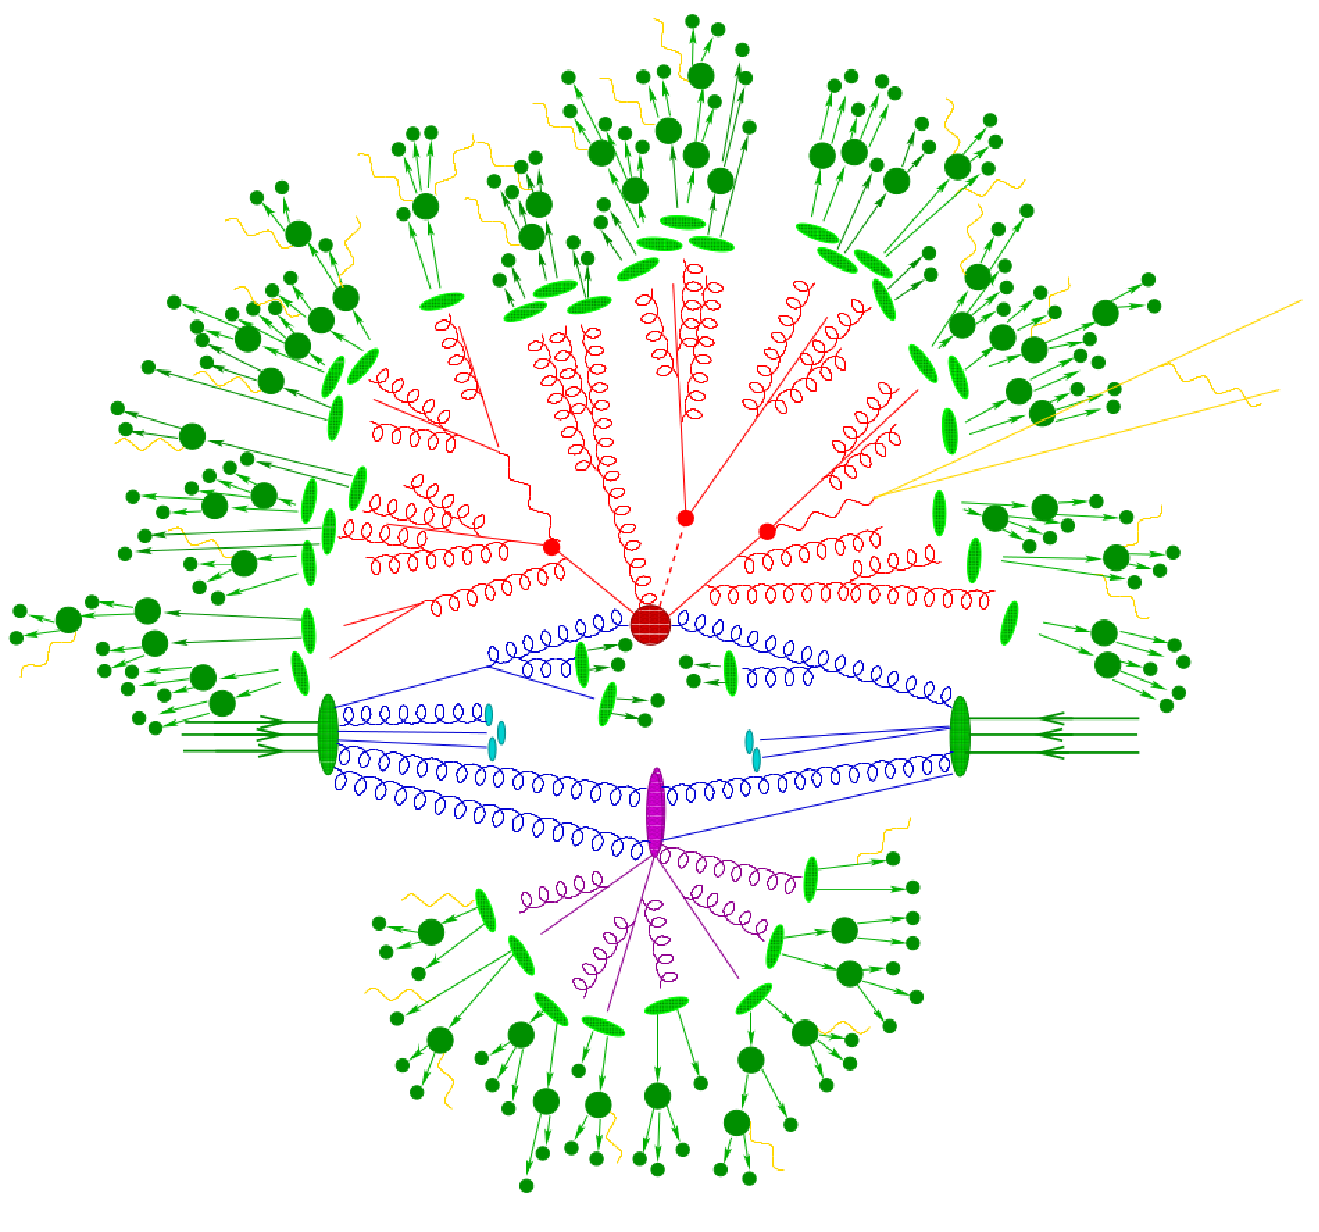
\includegraphics[width=1.0\linewidth]{Simulated_event.pdf}
    \caption{The simulation chain for a typical process at hadron colliders. The red blob in the center represents the hard collision, surrounded by a tree-like structure representing Bremsstrahlung as simulated by parton showers. The purple blob indicates a secondary hard scattering event. Parton-to-hadron transitions are represented by light green blobs, dark green blobs indicate hadron decays, while yellow lines signal soft photon radiation  \cite{2015introduction}.}
    \label{fig:Simulated_event}
\end{figure}
